\documentclass[UTF8]{ctexart}
\usepackage{algorithm}
\usepackage{algorithmic}
\usepackage{amsmath,amssymb}
\usepackage{booktabs}
\usepackage{geometry}
\usepackage{tikz}
\usepackage{color}

\geometry{a4paper,scale=0.7}

\renewcommand{\algorithmicrequire}{ \textbf{Input:}} %Use Input in the format of Algorithm
\renewcommand{\algorithmicensure}{ \textbf{Output:}} %UseOutput in the format of Algorithm

\begin{document}
    SA22225226 李青航

    ~\\
    \noindent\textbf{19.2-1}

    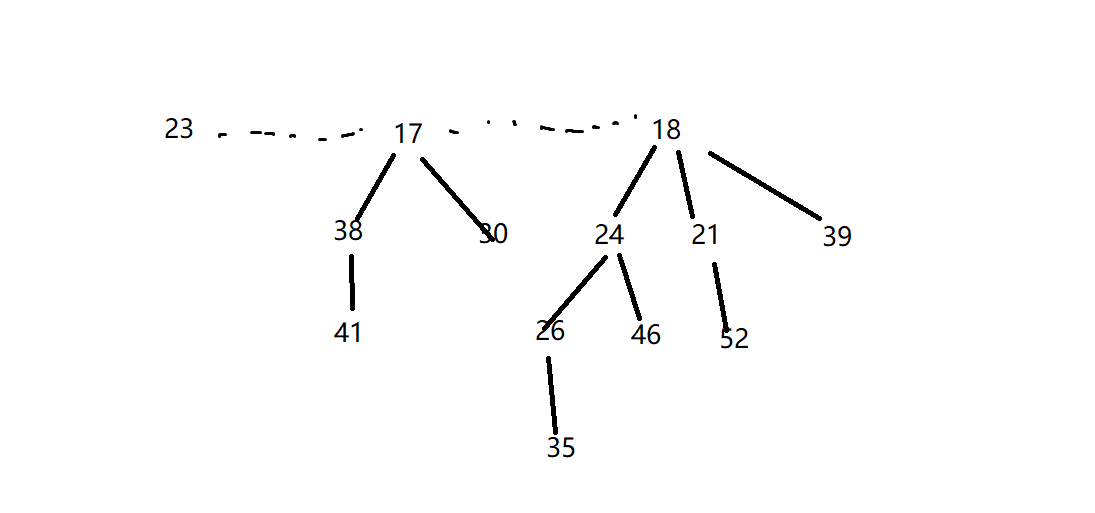
\includegraphics{1.png}

    ~\\
    \noindent\textbf{19.3-1}

    堆中的根被标记,因为它在某个时刻有一个子节点key的值被decreased。

    任何的进行的标记操作不会增加势。
    这是因为检查标记的唯一时间是在CASCADING-CUT的第3行。
    然而,这只会在其父节点为非NIL的节点上运行。
    因为每个根都有NIL作为它的父节点,
    所以CASCADING-CUT的第3行永远不会在这个标记的根上运行。
    
    ~\\
    \noindent\textbf{19.3-2}

    FIB-HEAP-DECREASE-KEY的实际开
    销是 $O(c)$ ,其中 $c$ 是调用CASCADING-CUT的次数。
    如果 $c_i$ 是对第 $i$ 个键进行调用的次数减少,
    那么对FIB-HEAP-DECREASE-KEY进行 $n$ 次调用的总时间
    为 $\sum ^{n}_{i=1}= O(c_i)$。接下来观察,
    对CASCADING-CUT的每一次调用都将一个节点移动到
    根节点,并且对根节点的每一次调用都需要 $O(1)$ 。
    因为在这些调用过程中没有根结点变成子结点,
    所以我们必须得到 $\sum ^{n}_{i=1} c_i = O(n)$ 。
    因此,总代价是O(n),所以平摊代价是O(1)。


\end{document}